\documentclass{beamer}

\usepackage{listings}
\usepackage{slashbox}
\usepackage{tikz}
\usepackage{booktabs}
\usepackage{amsmath,amssymb}
\usepackage{hyperref}
\usepackage{graphicx}

\DeclareMathOperator*{\argmin}{arg\,min}
\DeclareMathOperator*{\argmax}{arg\,max}
\DeclareMathOperator*{\maximize}{maximize}
\DeclareMathOperator*{\minimize}{minimize}
\newcommand{\sign}{\operatorname{sign}}
\newcommand{\RR}{\mathbb R}
\newcommand{\NN}{\mathbb N}

\AtBeginSection[]
{
  \begin{frame}
    \tableofcontents
  \end{frame}
}

\begin{document}

\title{Support vector comparison machines}
\author{
Toby Dylan Hocking\\
toby@sg.cs.titech.ac.jp\\
\url{http://sugiyama-www.cs.titech.ac.jp/~toby/}\\
joint work with Supaporn Spanurattana and Masashi Sugiyama
}

%\date{6 Aug 2013}

\maketitle

\section{Introduction and related work}

\begin{frame}
  \frametitle{Motivating example: learning to compare sushi}
  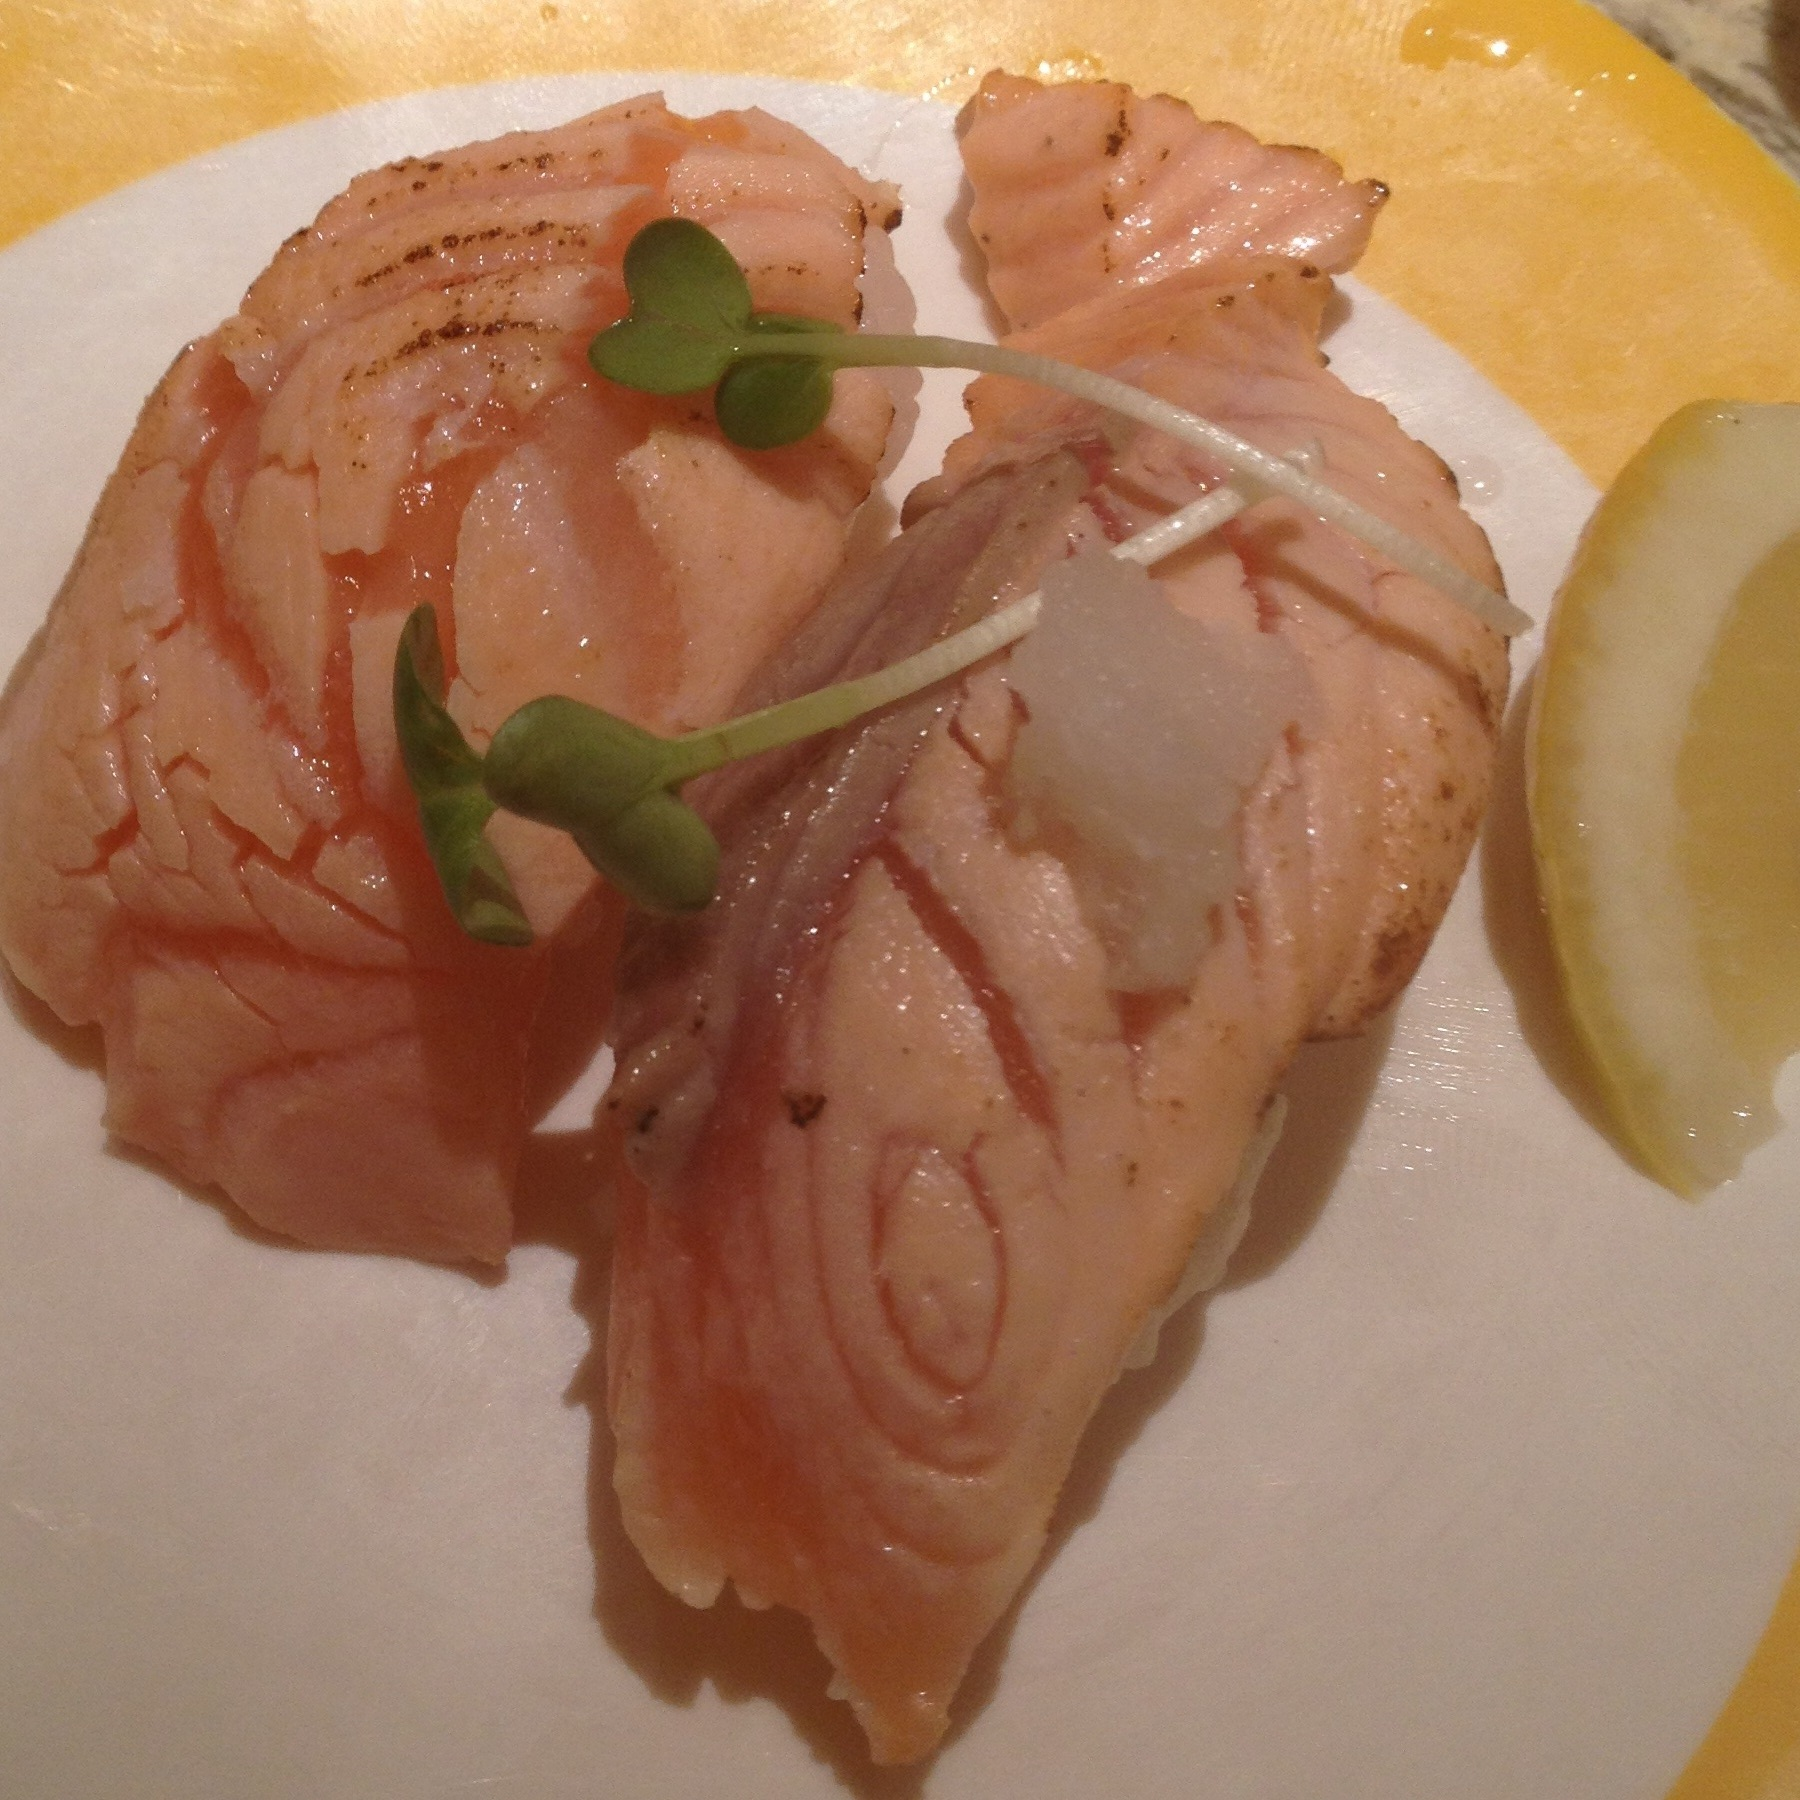
\includegraphics[width=1in]{sushi_salmon}\makebox[2.5in]{salmon is
    better than anago}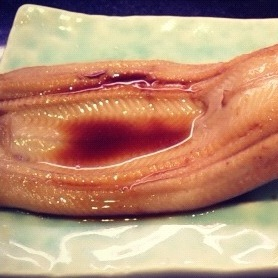
\includegraphics[width=1in]{sushi_anago}

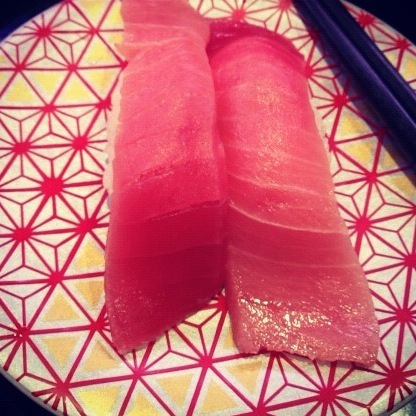
\includegraphics[width=1in]{sushi_chu-toro}\makebox[2.5in]{\alert<2>{chu-toro is
  as good as kani-miso}}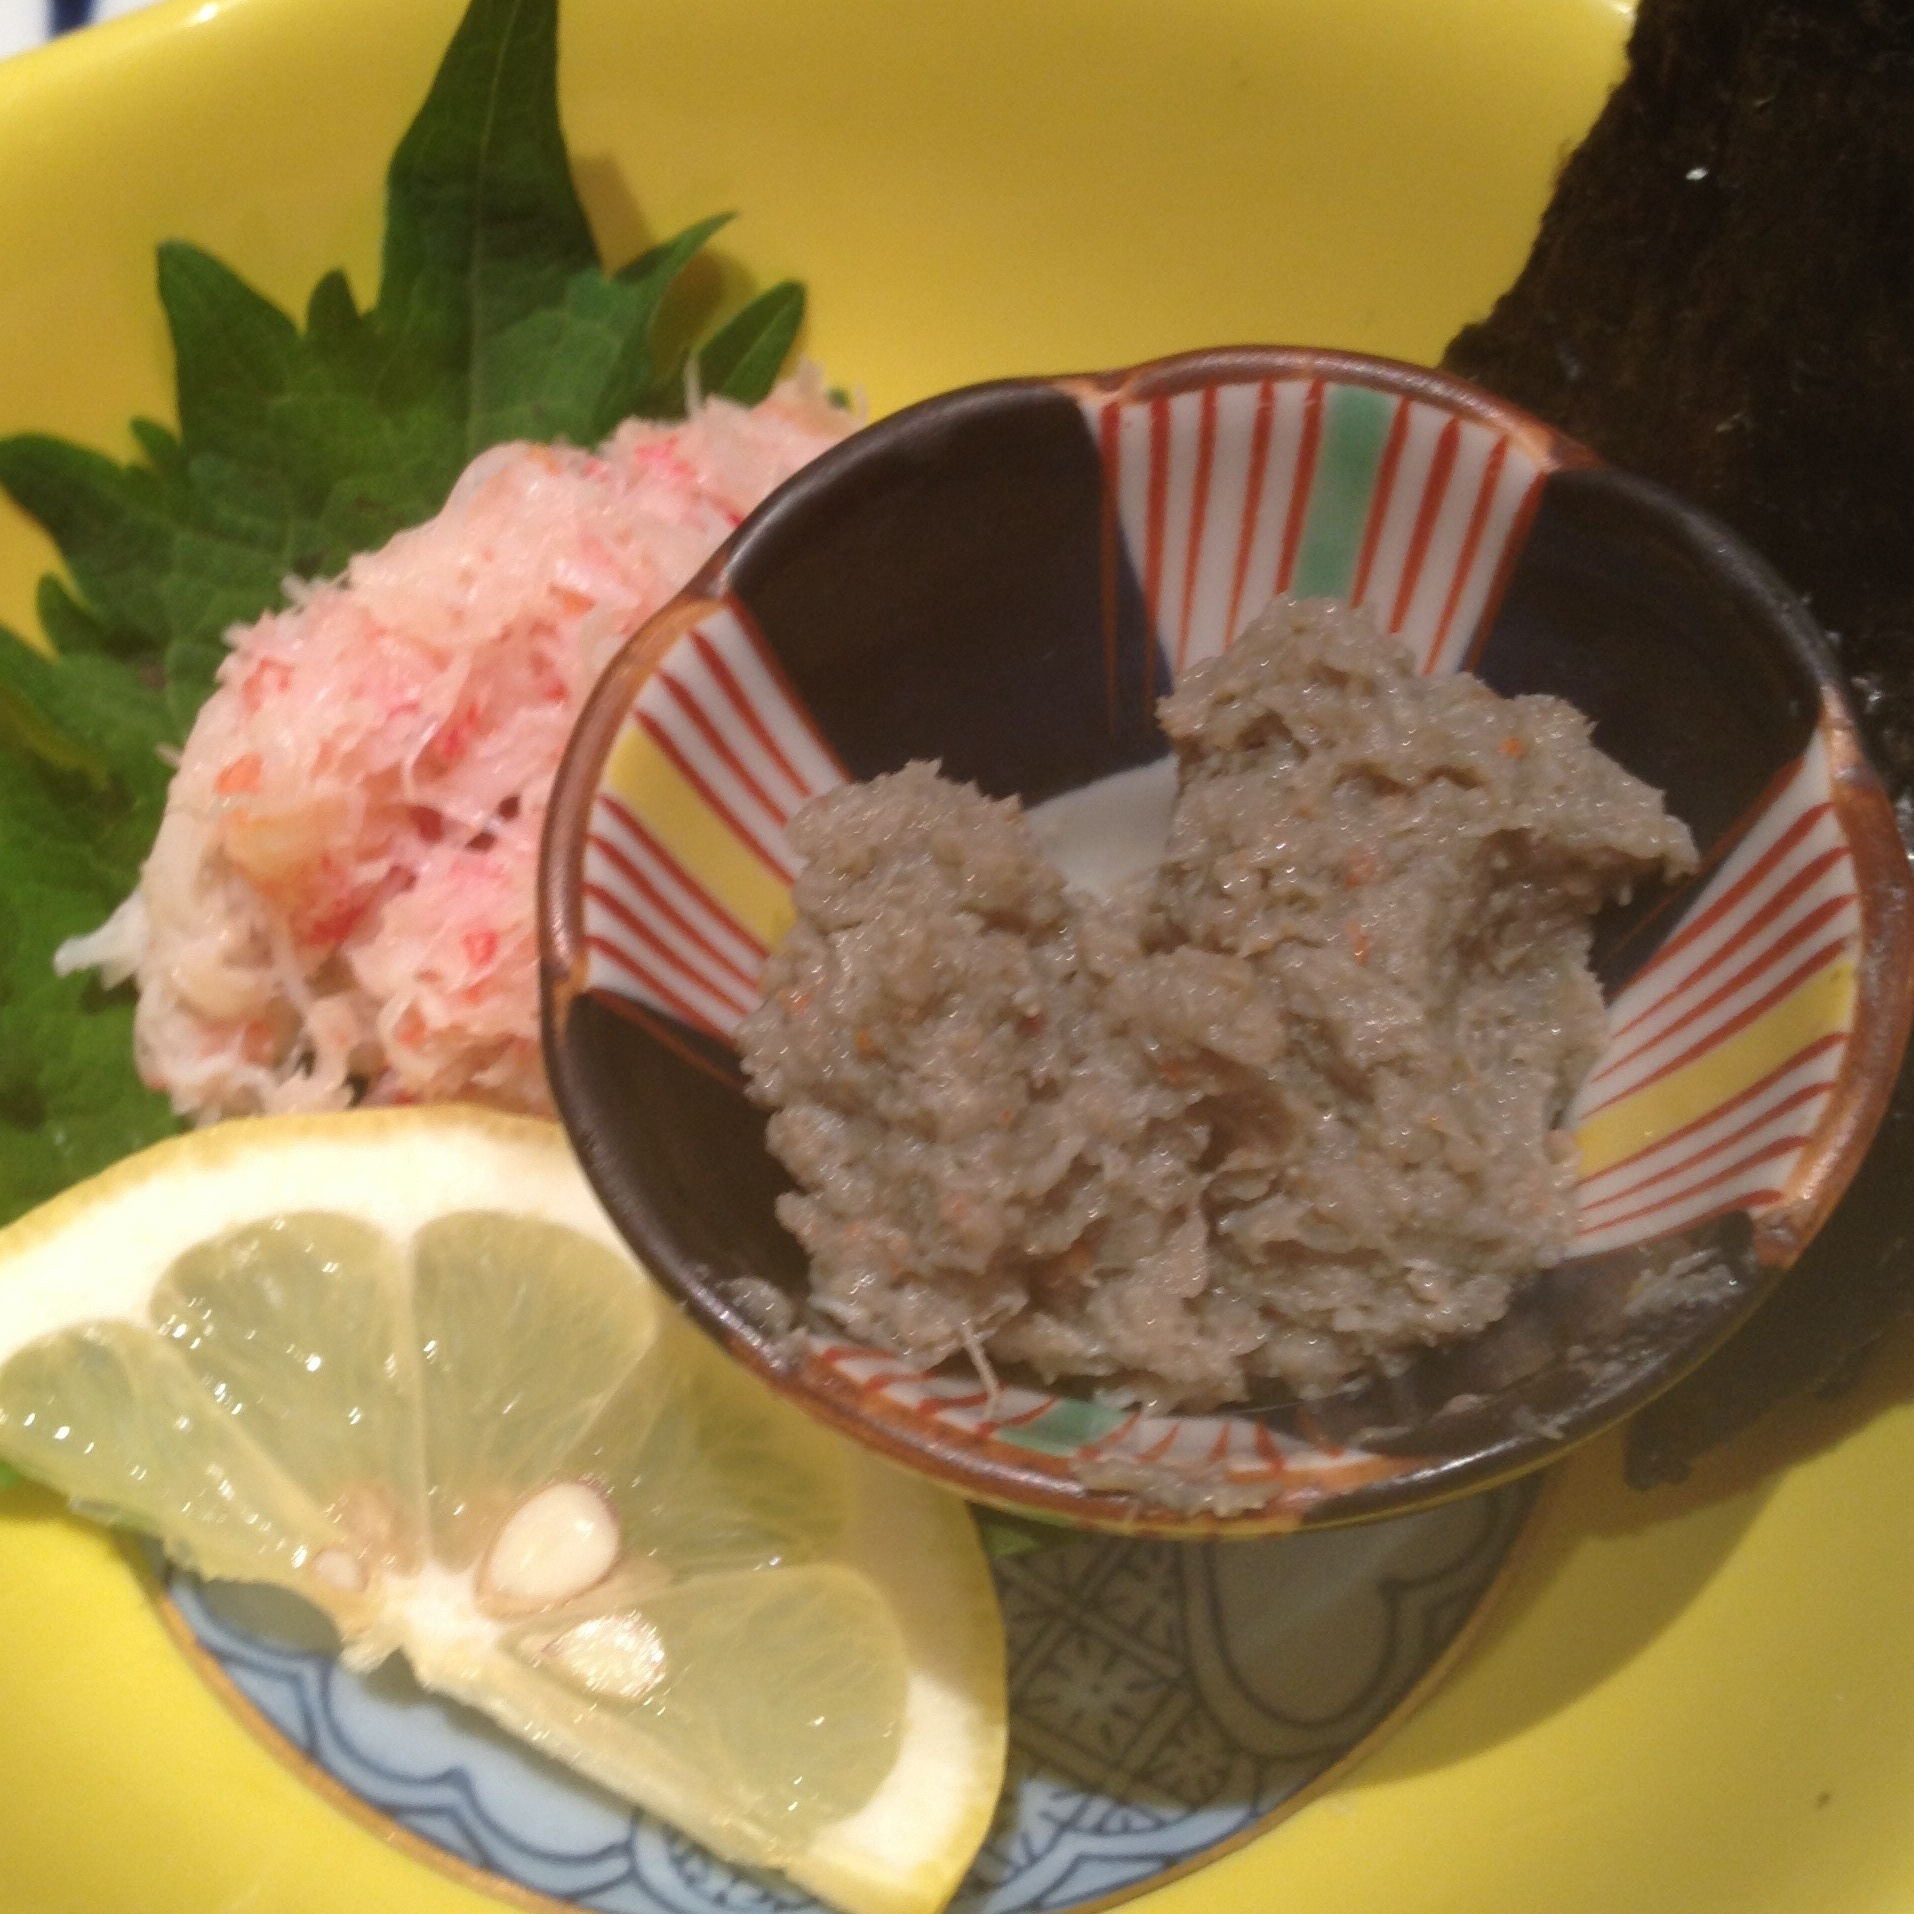
\includegraphics[width=1in]{sushi_kani-miso}

If I give you another sushi pair,\\
can you tell me which one is better,\\
\alert<2>{or if they are equally good?}
\end{frame}

\begin{frame}
  \frametitle{Learning a comparison function}
  We are given $n$ training pairs $(\mathbf x_i,\mathbf x_i',y_i)$ 
  \begin{itemize}
  \item Input: a pair of feature vectors $\mathbf x_i,\mathbf x_i'\in\RR^p$\\
    e.g. sushi fattiness, taster birthplace.
  \item Output: a label $y_i=
  \begin{cases}
    -1 & \text{ if $\mathbf x_i$ is better}\\
    0 & \text{ if $\mathbf x_i$ is as good as $\mathbf x'_i$}\\
    1 & \text{ if $\mathbf x'_i$ is better}.
  \end{cases}
$
  \end{itemize}
  Goal: find a comparison function
  $c:\RR^p\times\RR^p\rightarrow\{-1,0,1\}$
\begin{itemize}
\item Good prediction with respect to the zero-one loss:
$$\minimize_c \sum_{i\in\text{test}} 
I\left[ y_i \neq c(\mathbf x_i,\mathbf x_i') \right]$$
\item Symmetry: $c(\mathbf x,\mathbf x') = -c(\mathbf x',\mathbf x)$.
\end{itemize}
\end{frame}

\begin{frame}
  \frametitle{Geometric interpretation when $r(\mathbf x)=||\mathbf
    x||_2^2$}
  \begin{minipage}{1.0\linewidth}
    \hskip -0.5cm
      \input{figure-geometry}
  \end{minipage}
\end{frame}

\begin{frame}
  \frametitle{Geometric interpretation when $r(\mathbf x)=||\mathbf
    x||_2^2$}
  \begin{minipage}{1.0\linewidth}
    \hskip -0.5cm
  \input{figure-norm-data}
  \end{minipage}
\end{frame}

\begin{frame}
  \frametitle{Related work: reject, rank, and rate}
\renewcommand{\arraystretch}{1.5}
\begin{tabular}{|c|c|c|}\hline
  \backslashbox{Outputs}{Inputs}
  &single items $\mathbf x$&pairs of items $\mathbf x,\mathbf x'$\\ \hline
  $y\in\{-1,1\}$ &SVM  & SVMrank   	\\ \hline 
  $y\in\{-1,0,1\}$ &Reject option& this work\\ \hline
\end{tabular}
\begin{itemize}
\item PL Bartlett and MH Wegkamp. Classification with a reject
  option using a hinge loss. JMLR, 9:1823--1840, 2008. (statistical
  properties of the hinge loss)
\item T Joachims. Optimizing search engines using clickthrough
  data. KDD 2002. (SVMrank)
\item K Zhou \emph{et al.} Learning to rank with ties. SIGIR
  2008. (boosting, ties are more effective with more output values)
\item R Herbrich \emph{et al.} TrueSkill: a Bayesian skill rating
  system. NIPS 2006. (generalization of Elo for chess)
\end{itemize}
\end{frame}

\begin{frame}
  \frametitle{SVMrank is a quadratic program (QP)}
  \begin{equation*}
    \begin{aligned}
          \minimize_{\mathbf w\in\RR^p}\ \  & \mathbf w^\intercal \mathbf w \\
          \text{subject to}\ \  & 
          \mathbf w^\intercal(\mathbf x_i'-\mathbf x_i)y_i \geq 1,
          \ \forall i\in \mathcal I_1\cup \mathcal I_{-1}.
    \end{aligned}
  \end{equation*}
  \input{figure-max-margin-bothsides-svmrank}
Note: $y_i=0$ equality pairs are not used!
\end{frame}

\section{Learning a max-margin comparison function}

\begin{frame}
  \frametitle{Learning to rank and compare}
  We will learn a
  \begin{itemize}
  \item Ranking function $r:\RR^p\rightarrow\RR$. Bigger is better.
  \item Threshold $\tau\in\RR^+$. \\A small difference
    $|r(\mathbf x')-r(\mathbf x)|\leq \tau$ is not significant.
  \item Comparison function $c_\tau(\mathbf x, \mathbf x') =
  \begin{cases}
    -1 & \text{ if }r(\mathbf x')-r(\mathbf x) < -\tau\\
    0 & \text{ if }|r(\mathbf x')-r(\mathbf x)|\leq \tau\\
    1 & \text{ if }r(\mathbf x')-r(\mathbf x) > \tau.
  \end{cases}
$
\end{itemize}
The problem becomes
$$\minimize_{r,\tau} \sum_{i=1}^n 
I\left[ y_i\neq c_\tau(\mathbf x_i, \mathbf x_i') \right].$$
\end{frame}

\begin{frame}
  \frametitle{Max margin comparison is a linear program (LP)}
  For $y\in\{-1,0,1\}$, let $\mathcal I_y=\{i\mid y_i=y\}$ be the
  corresponding training indices.
  \begin{equation*}
  \begin{aligned}
    \maximize_{\mu\in\RR, \mathbf w\in\RR^p}\ & \mu \\
    \text{subject to}\ & 
    \mu \leq 1-|\mathbf w^\intercal (\mathbf x_i' - \mathbf x_i)|,\
    \forall\  i\in \mathcal I_0\\
    &\mu \leq -1 +  
    \mathbf w^\intercal(\mathbf x_i'-\mathbf x_i)y_i,
    \ \forall\ i\in \mathcal I_1\cup \mathcal I_{-1}.
  \end{aligned}
\end{equation*}
Note: if the optimal $\mu>0$ then the data are separable.
\end{frame}

\section{Results and conclusions}

\begin{frame}
  \frametitle{Simulation: true patterns $r$ and noisy training pairs}
  \begin{minipage}{1.0\linewidth}
    \hskip -0.5cm \input{figure-truth-train} Validation and test data
    have the same number of pairs $n$ and the same proportion of
    equality pairs $\rho$.
  \end{minipage}
\end{frame}

\begin{frame}
  \frametitle{Details of simulation setup}
  \begin{itemize}
    \item Inputs $\mathbf x_i,\mathbf x_i'\in[-3,3]^2$.
    \item True ranking function $r(\mathbf x)=||\mathbf x||^2_j$ 
      for $j\in\{1,2,\infty\}$.
    \item Noisy labels $y_i=t_1[r(\mathbf x'_i)-r(\mathbf x_i)+\epsilon_i]$.
  \item Threshold function
$
  \label{eq:threshold}
  t_1(x) = 
  \begin{cases}
    -1 & \text{ if } x < -1, \\
    0 & \text{ if } |x| \leq 1, \\
    1 & \text{ if } x > 1. \\
  \end{cases}
$
\item Noise $\epsilon_i\sim N(0, \sigma)$ with standard deviation
  $\sigma=1/4$.
\item Train, validation, and test sets with
  \begin{itemize}
    \item same number of training pairs $n$, and
    \item same proportion of equality pairs $\rho$.
  \end{itemize}
\item Fit a $10\times 10$ grid of models to the training
set:
\begin{itemize}
\item Cost parameter $C=10^{-3},\dots,10^3$,
\item Gaussian kernel width $2^{-7},\dots,2^4$.
\end{itemize}
\item Select the model with minimal zero-one loss on the validation set.
  \end{itemize}
\end{frame}

\begin{frame}
  \frametitle{We ran 3 different algorithms on each data set}
  \begin{center}
        \begin{tabular}{r|cc|cc|c|}
&    \multicolumn{2}{c|}{equality pairs}
&    \multicolumn{2}{c|}{inequality pairs}\\
Input:    & $|\mathcal I_0|$ %$\tilde y_i= -1$
    & --- 
    & $|\mathcal I_1|+|\mathcal I_{-1}|$ %$\tilde y_i=1$
    & $\rightarrow$ &
    code
    \\
    \hline
    rank 
    & 0 
    & 
    & $|\mathcal I_1|+|\mathcal I_{-1}|$ 
    & $\rightarrow$ &
    SVMrank
    \\
    \hline
    rank2 
    & $2|\mathcal I_0|$ 
    & $\leftarrow \rightarrow$
    & $2(|\mathcal I_1|+|\mathcal I_{-1}|)$ 
    & $\rightarrow \rightarrow$ &
    SVMrank
    \\
    \hline
    compare 
    & $2|\mathcal I_0|$ 
    & --- --- 
    & $|\mathcal I_1|+|\mathcal I_{-1}|$ 
    & $\rightarrow$ &
    proposed
    \\
    \hline
  \end{tabular}
  \end{center}
  \begin{description}
  \item[Equality $y_i=0$ pairs] are shown as ---  
    segments.
  \item[Inequality $y_i\in\{-1,1\}$ pairs]
    are shown as $\rightarrow$  arrows.
  \item[rank] ignores each input equality pair.
  \item[rank2] converts each input equality pair
    to two contradictory inequality pairs.
  \item[compare] directly models the equality pairs.
  \end{description}
\end{frame}

%\input{sample-level-curves}

\begin{frame}
  \frametitle{Test error lowest for proposed SVMcompare model}
  \begin{minipage}{1.0\linewidth}
    \hskip -0.5cm
      \input{figure-simulation-samples-linf}
  \end{minipage}
\end{frame}

\begin{frame}
  \frametitle{Test error lowest for proposed SVMcompare model}
  \begin{minipage}{1.0\linewidth}
    \hskip -0.5cm
      \input{figure-simulation-samples}
  \end{minipage}
\end{frame}

%\input{proportion-level-curves}

\begin{frame}
  \frametitle{No difference for few equality pairs,\\
    rank worse when there are many equality pairs}
  \begin{minipage}{1.0\linewidth}
    \hskip -0.5cm
      \input{figure-auc-linf}
  \end{minipage}
\end{frame}

\begin{frame}
  \frametitle{No difference for few equality pairs,\\
    rank worse when there are many equality pairs}
  \begin{minipage}{1.0\linewidth}
    \hskip -0.5cm
      \input{figure-auc}
  \end{minipage}
\end{frame}

\begin{frame}
  \frametitle{Sushi data of Kamishima et al.}
  \begin{itemize}
  \item  \url{http://www.kamishima.net/sushi/}
  \item 100 different sushis rated by 5000 different people.
  \item Each person rated 10 sushis on a 5 point scale. 
  \item Convert 10 ratings to 5 preference pairs.
  \item 17,832 equality $y_i=0$ pairs and
  \item 7,168 inequality $y_i\in\{-1,1\}$ pairs.
  \item Feature pairs $\mathbf x_i,\mathbf x_i'\in\RR^{14}$.
  \item 7 sushi features: style, major, minor, oily, eating frequency,
    price, and selling frequency.
  \item 7 taster/person features: Sushi gender, age, time, birthplace
    and current home (we converted Japanese prefecture codes to
    latitude/longitude coordinates).
  \end{itemize}
\end{frame}

\begin{frame}
  \frametitle{Sushi data are harder,\\
    but SVMcompare still has lowest test error}
  \begin{minipage}{1.0\linewidth}
    \hskip -1cm
      \input{figure-sushi}
  \end{minipage}
\end{frame}

\begin{frame}
  \frametitle{Conclusions and future work}
  \begin{itemize}
  \item Learned a nonlinear ranking function $r(\mathbf x)\in\RR$, and
  \item a comparison function $c(\mathbf x, \mathbf x')\in\{-1,0,1\}$.
  \item Results: rank $<$ rank2 $<$ compare.
  \item Directly learning from $y_i=0$ equality pairs is important,\\
    when they are present!
  \item \url{https://github.com/tdhock/rankSVMcompare}
  \item Scaling to large data? Stochastic gradient methods?
  \end{itemize}
\end{frame}

\begin{frame}
  \frametitle{Thank you!}
  Supplementary slides appear after this one.
\end{frame}

\end{document}
